\begin{frame}[fragile]
    \begin{definition}[quadratic closed field]
        \label{def:quadritc_closed_field}
        \leanok
        \lean{QuadraticClosed}
        A field $F$ is called \emph{quadratic closed} if for all $x \in F$ there is a $y \in F$ such that $y^2 = x$.
    \end{definition}

    \begin{lemma}
        \label{lem:M_inf_quad_closed}
        \leanok
        \lean{MField_QuadraticClosed, MField_QuadraticClosed_def}
        \uses{def:set_of_constructable_points, def:quadritc_closed_field}
        For $M\subseteq \mathbb{C}$ with $0,1 \in M$, $M_{\infty}$ is quadratic closed.
    \end{lemma}
    \pause
    \begin{proof}
        \begin{enumerate}
            \item The root of $r\in \R_{\ge 0}$/$r\in \R_{\ge 1}$ is in $M_{\infty}$.
            \pause
            \item If $e^{i\alpha}\in M_{\infty}$ then $e^{i\alpha/2}\in M_{\infty}$.
            \pause
            \item If $z\in M_{\infty}$ then ther exists $r, e^{i\alpha}\in M_{\infty}$ such that $z = r e^{i\alpha}$.
        \end{enumerate}
    \end{proof}
\end{frame}

\begin{frame}[fragile]
    \frametitle{1. The root of $r\in \R_{\ge 0}$/$r\in \R_{\ge 1}$ is in $M_{\infty}$.}
    w.l.o.g we can assume that $r\in \R_{\ge 1}$, since $root(r) = \frac{1}{\sqrt{r^{-1}}}$.
    \scalebox{0.8}{\begin{minipage}{1.20\textwidth}

        \begin{figure}
        \centering
        \begin{tikzpicture}
            \draw[->] (-1,0) -- (7,0) node[right] {$\Re$};
            \draw[->] (0,-1) -- (0,4) node[above] {$\Im$};
            \coordinate[label=-135:$0$] (zero) at (0,0);
            \coordinate[label=-90:$1$] (one) at (1,0);
            \coordinate[label=-45:$r$] (r) at (6,0);
            \coordinate[label=-90:$\frac{r}{2}$] (r2) at (3,0);
            \coordinate[label=135:] (sqrt1) at (1,2.2360679775);
            \coordinate[label=135:$\sqrt{r}$] (sqrt) at (2.4494897428,0);
            \fill[black] (zero) circle (1pt);
            \fill[black] (one) circle (2pt);
            \fill[black] (r) circle (2pt);
            \fill[black] (r2) circle (2pt);
            \fill[black] (sqrt1) circle (2pt);
            \draw (r2) [carc=-10:190:3];
            \draw (zero) [carc=-10:80:2.4494897428];
            \draw (one) -- (sqrt1);
            \fill[red] (sqrt) circle (3pt);
        \end{tikzpicture}
        \caption{Construction of $\sqrt{r}$}
        \label{Fig.root}
        \end{figure}
    
        \end{minipage}}
\end{frame}
    
\begin{frame}
    \frametitle{2. If $e^{i\alpha}\in M_{\infty}$ then $e^{i\alpha/2}\in M_{\infty}$.}
    \begin{columns}
    
        \begin{column}{0.5\textwidth}
            \begin{figure}[h]
                \centering
                \begin{tikzpicture}
                    \draw[->] (-0.5,0) -- (2.5,0) node[right] {$\Re$};
                \draw[->] (0,-0.5) -- (0,2.5) node[above] {$\Im$};
                \coordinate[label=-135:$0$] (zero) at (0,0);
                \fill[black] (zero) circle (2pt);
                \coordinate[label=-90:$1$] (one) at (2,0);
                \fill[black] (one) circle (2pt);
                \coordinate[label=-180:$e^{\imath\alpha}$] (e) at (0,2);
                \fill[black] (e) circle (2pt);
                \draw[dashed] (e) -- (one);
                \draw (zero) [carc=-10:100:2];
                \node (X) at (1,1) {X};
                \coordinate[label=45:$e^{\imath\alpha/2}$] (e2) at (1.42,1.42);
                \fill[black] (e2) circle (2pt);
                \draw (zero) -- (e2);
                
                \end{tikzpicture}
            \end{figure}

        \end{column}
        \begin{column}{0.5\textwidth}
            \begin{itemize}
                \item case $\alpha = 0$ or $\alpha = \pi$
                \item Remark: Midpoint is constructable % field and addition divition two
                \item Intersection of the unit circle with the line passing through $0$ and the midpoint of $1$ and $e^{\imath \alpha}$.
                \item calculate that it is the right point
            \end{itemize}
        \end{column}
    \end{columns}

\end{frame}

\begin{frame}[fragile]
    \frametitle{3. If $z\in M_{\infty}$ then ther exists $r, e^{i\alpha}\in M_{\infty}$}
\begin{columns}
    
    \begin{column}{0.5\textwidth}
        Using 1) and $r = \sqrt{\Re(z)^2+\Im(z)^2} $
        \begin{figure}[h]
            \centering
            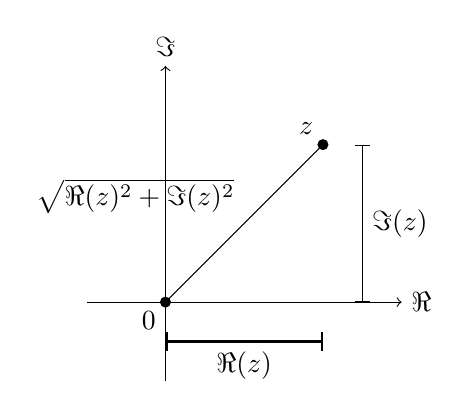
\begin{tikzpicture}
            
                \draw[->] (-1,0) -- (3,0) node[right] {$\Re$};
                \draw[->] (0,-1) -- (0,3) node[above] {$\Im$};
                \coordinate[label=-135:$0$] (zero) at (0,0);
                \fill[black] (zero) circle (2pt);
                \coordinate[label=135:$z$] (z) at (2,2);
                \fill[black] (z) circle (2pt);
                \coordinate[label=135:$\sqrt{\Re(z)^2+\Im(z)^2}$] (sprt) at (1,1);
                \draw (zero) -- (z);
                \draw[thick, style={ |-|}] (0,-0.5) -- (1,-0.5)  node[below] {$\Re(z)$} -- (2,-0.5);
                \draw[ style={ |-|}] (2.5,0) -- (2.5,1)  node[right] {$\Im(z)$} -- (2.5,2);
            \end{tikzpicture}
        \end{figure}
    
    \end{column}
    \pause
    \begin{column}{0.5\textwidth}
        \begin{figure}[h]
            \centering
            \begin{tikzpicture}
                \draw[->] (-0.5,0) -- (4,0) node[right] {$\Re$};
                \draw[->] (0,-0.5) -- (0,3) node[above] {$\Im$};
                \coordinate[label=-135:$0$] (zero) at (0,0);
                \coordinate[label=-135:$1$] (one) at (1,0);
                \coordinate[label=135:$z$] (z) at (3,2);
                \coordinate[label=90:$e^{\imath\alpha}$] (ea) at (0.8321,0.5547);
                \fill[black] (zero) circle (1pt);
                \fill[black] (one) circle (2pt);
                \fill[black] (z) circle (2pt);
                \fill[black] (ea) circle (2pt);
                \draw (zero) -- (z);
                \draw (zero) [carc=-20:110:1];
            \end{tikzpicture}
            \caption{Construction of $e^{\imath\alpha}$}
            \label{Fig.angle}
        \end{figure}
    \end{column}
\end{columns}

\end{frame}

\begin{frame}
    \begin{definition}
        \label{def:conj_set}
        \leanok
        \lean{conj_set}
        For a Set $M \subset \mathbb{C}$ we define the \emph{conjugate set} of $M$ as 
        \begin{equation*}
            Conj(M) = \{\overline{z}\mid z\in M\}
        \end{equation*}
    \end{definition}
    
    \begin{definition}
        \label{def:conj_closed}
        \leanok
        \lean{ConjClosed}
        \uses{def:conj_set}
        We call a subset of $\C$ \emph{conjugate closed} if $M= Conj(M)$.
    \end{definition}
\end{frame}

\begin{frame}
    \begin{theorem}
        Let $K$ be an conjugation closed intermediate field of $\mathbb{Q}$ and $\mathbb{C}$.
        \begin{enumerate}
            \item If $z\in ill(K)$ then $z\in K$.
            \item If $z\in ilc(K)$ then there exist $w^2 \in K$ such that $z\in K(w)$.
            \item If $z\in icc(K)$ then there exist $w^2 \in K$ such that $z\in K(w)$.
        \end{enumerate}
    \end{theorem}
\end{frame}

\begin{frame}
    
    \begin{lemma}[2]
        \label{lem:ConjClosed.Intersection_line_circle}
        \leanok
        \uses{def:conj_closed}
        Let $L$ be a subfield of $\mathbb{C}$, with $L = conj(L)$. For $i = 1,2,3$ let $z_i = x_i + \imath y_i \in L$ with $z_1 \ne z_2$, and let $r > 0$ in $\mathbb{R}$ with $r^2 \in L$. Define
        \begin{equation*}\begin{aligned}
            G := \{\lambda z_1 + (1-\lambda)z_2 \mid \lambda \in \mathbb{R}\},\\
            C := \{z = x + \imath y \in \mathbb{C} \mid \|z - z_3\| = r\}.
        \end{aligned} \end{equation*}
        Assume $G \cap C \ne \emptyset$; then the following are equivalent:
        \begin{itemize}
            \item $z\in G \cap C$.
            \item There is a $\lambda \in \mathbb{R}$ with $\lambda^2 a+ \lambda b + c = 0$ where
            \begin{align*}
                a &:= (x_1 - x_2)^2 + (\imath y_1 - \imath y_2)^2,\\
                b &:= 2(x_1 - x_2)(x_2 - x_3) - 2(\imath y_1 - \imath y_2)(\imath y_2 - \imath y_3),\\
                c &:= (x_2 - x_3)^2 + (\imath y_2 - \imath y_3)^2 - r^2,
            \end{align*}
            and $z = \lambda z_1 + (1-\lambda)z_2$.
        \end{itemize}
        In this case $z \in L(\sqrt{w})$ for an $w \in L$.
    \end{lemma}
\end{frame}

\begin{frame}
    \frametitle{Proof of 2}
    \scalebox{0.8}{\begin{minipage}{1.2\textwidth}

    \begin{align*}
        &&\|z - z_3\| &= r &&\mid 0\le \|\cdot\|\text{ and }0\le r\\
        &\Leftrightarrow& \|z - z_3\|^2 &= r^2\\
        &\Leftrightarrow& (x - x_3)^2 + (\imath y - \imath y_3)^2 &= r^2 &&\mid x = \lambda x_1 - \lambda x_2 + x_2 \text{ and }\\ 
        &&&&&\mid y = \lambda y_1 - \lambda y_2 + y_2\\
        &\Leftrightarrow& (\lambda x_1 - \lambda x_2 + x_2 - x_3)^2 + \\
        &&(\imath (\lambda y_1 - \lambda y_2 + y_2 - y_3))^2 &= r^2\\
        &\Leftrightarrow& \lambda ^2 ((x_1 - x_2)^2 + (\imath y_1 - \imath y_2)^2) + \\
        &&\lambda (2(x_1 - x_2)(x_2 - x_3) - 2(\imath y_1 - \imath y_2)(\imath y_2 - \imath y_3)) + \\
        &&(x_2 - x_3)^2 + (\imath y_2 - \imath y_3)^2 &= r^2\\
    \end{align*}
    \end{minipage}}
\end{frame}

\begin{frame}
    \frametitle{Proof of 2}
    \begin{itemize}
        \item $z = \lambda z_1 + (1-\lambda)z_2$.
        \item $lambda$ is root of $a X^2 + b X + c$.
        \item [$\Rightarrow$] $lambda\in L(\sqrt{w}) = \frac{-b \pm \sqrt{b^2 - 4ac}}{2a}$
        \item [$\Rightarrow$] $z\in L(\sqrt{w})$ for $w = b^2 - 4ac \in L$
    \end{itemize}
\end{frame}
